\item An infinitely long thin non-conducting wire is parallel to the z-axis and carries a uniform line charge density $\lambda$. It pierces a thin non-conducting spherical shell of radius $R$ in such a way that the arc $PQ$ subtends an angle $120^\circ$ at the centre $O$ of the spherical shell, as shown in the figure. The permittivity of free space is $\varepsilon_0$. Which of the following statements is (are) true?
\begin{center}
    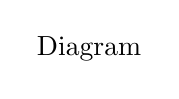
\begin{tikzpicture}
        \node {Diagram};
    \end{tikzpicture}
\end{center}
    \begin{tasks}(1)
        \task The electric flux through the shell is $\sqrt{3}R\lambda/\varepsilon_0$
        \task The $z$-component of the electric field is zero at all the points on the surface of the shell
        \task The electric flux through the shell is $\sqrt{2}R\lambda/\varepsilon_0$
        \task The electric field is normal to the surface of the shell at all points
    \end{tasks}
